\chapter{Authorization}

\section{Introduction}

\url{https://helgeklein.com/blog/permissions-a-primer-or-dacl-sacl-owner-sid-and-ace-explained/#dissecting-security-descriptors-sd}

the following
\href{https://docs.microsoft.com/en-us/windows/security/identity-protection/access-control/security-principals}{picture}
diagram illustrates the Windows authorization and access control process.
\begin{figure}
  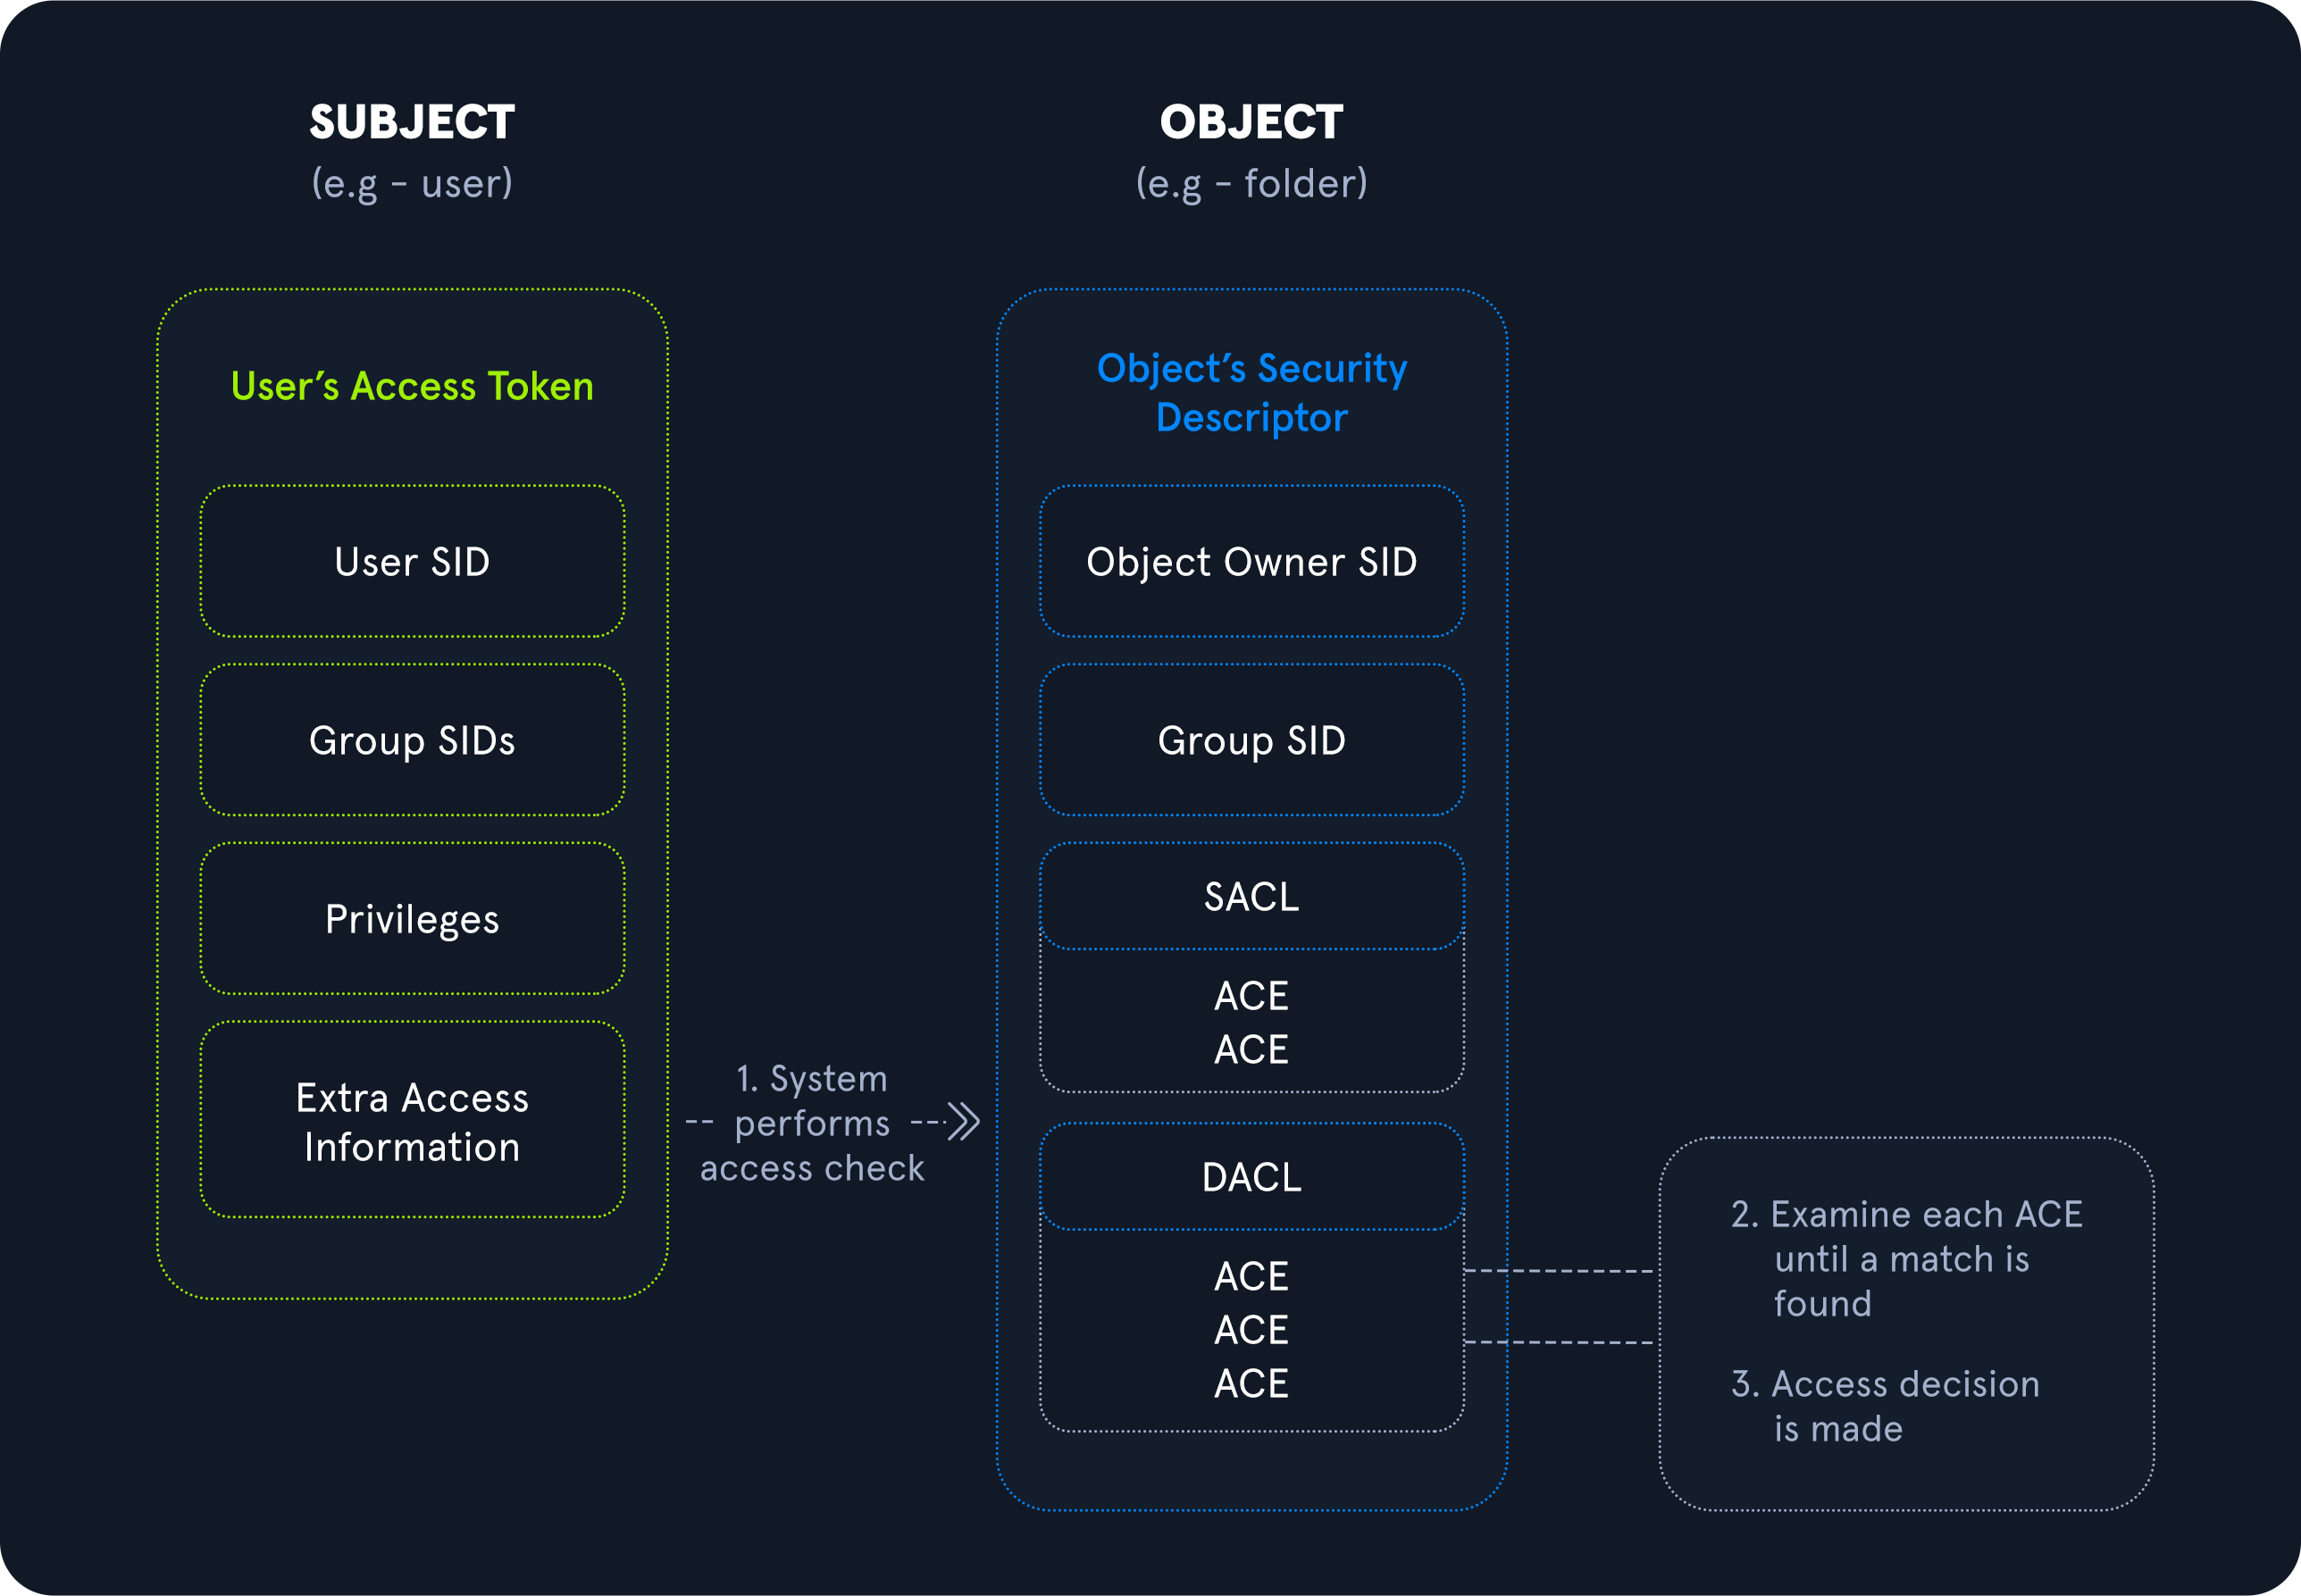
\includegraphics[width=\linewidth]{windows_knowledge/authorization/images/auth_process.png}
  \caption{Authorization process}
  \label{fig:authoriation process}
\end{figure}


Every object that can have a security descriptor (SD) is a
\href{https://docs.microsoft.com/en-us/windows/win32/secauthz/securable-objects}{securable object}
that may be protected by permissions. All named and several unnamed Windows
objects are securable and can have SDs, although this is not widely known.
There does not even exist a GUI for manipulating the SDs of many object types!
Have you ever tried to kill a system process in Task Manager and got the
message “Access denied”? This is due to the fact that this process’ SD does not
allow even administrators to kill the process. But it is, of course, possible,
as an administrator, to obtain the necessary permissions, provided a GUI or
some other tool is available.

\section{Securable Object}
\index{Windows!Securable Object}
\label{win:securable-object}

Among many others, the following object types are securable:
\begin{itemize}
        \item Files and directories on NTFS volumes
        \item Registry keys (but not values)
        \item Network shares
        \item Printers
        \item Services
        \item Active Directory objects
        \item Processes
\end{itemize}

Of these types, some are hierarchical in nature (directories, registry keys, …), and some are not (printers, services, …).


\section{Security Identifier (SID)}
\label{win:security-identifier}
\index{Windows!Security Identifier(SID)}

Each of the security principals on the system has a unique \emph{security
identifier (SID)}. The system automatically generates SIDs. This means that
even if, for example, we have two identical users on the system, Windows can
distinguish the two and their rights based on their SIDs. SIDs are string
values with different lengths, which are stored in the security database. These
SIDs are added to the user's \emph{access token}~\ref{win:access-token} to identify all actions that
the user is authorized to take.

A SID consists of the \emph{Identifier Authority} and the \emph{Relative ID
(RID)}. In an Active Directory (AD) domain environment, the SID also includes
the \emph{domain SID}.

The SID is broken down into this pattern:
\begin{verbatim}
(SID)-(revision level)-(identifier-authority)-(subauthority1)-(subauthority2)-(etc)
\end{verbatim}


Let's break down the SID piece by piece:

\begin{tabularx}{\linewidth}{|l|l|X|}
    \hline
Number &	Meaning &	Description\\
    \hline
S &	SID & Identifies the string as a SID.\\
    \hline
1 &	Revision Level &	To date, this has never changed and has always been
1.\\
    \hline
5 &	Identifier-authority &	A 48-bit string that identifies the authority (the
computer or network) that created the SID.\\
    \hline
21 &	Subauthority1 &	This is a variable number that identifies the user's
relation or group described by the SID to the authority that created it. It
tells us in what order this authority created the user's account.\\
    \hline
    67\ldots-40\ldots-20\ldots &	Subauthority2 &	Tells us which computer (or
domain) created the number\\
    \hline
1002 &	Subauthority3 &	The RID that distinguishes one account from another.
Tells us whether this user is a normal user, a guest, an administrator, or part
of some other group\\
    \hline
\end{tabularx}

\subsection{SID to Name Lookup}

It is important to remember that trustees referenced in
Security Descriptors~\ref{win:security-descriptor} are always stored
as binary SIDs. This is true for the owner, the primary group, and any trustee
in any access control list (ACL) (DACL~\ref{win:DACL} or SACL~\ref{win:DACL}) . This implies that there exists some mechanism
that converts trustee names into SIDs and vice versa. This mechanism is a
central part of the \emph{Security Accounts Mmanager (SAM)}~\ref{win:SAM} and of
the \emph{NTDS database}~\ref{win:NTDS}. The former manages the local account database on any NT-based system
(Windows NT right up to Windows 10, including the server variants). The latter
is only available on Active Directory Domain Controllers where it replaces the
SAM.

\subsection{Special SID: Capability SIDs}
Introduced by Windows 8 
\href{https://docs.microsoft.com/en-us/troubleshoot/windows-server/windows-security/sids-not-resolve-into-friendly-names}{Capability SIDs}
are used to grant applications access to resources such as the camera, or
the location.  They cannot be resolved to/from names, they are displayed as SID
strings in permission listings. Windows ACL Editor cannot add capability SIDs,
it can only delete them. To add them back use SetACL, specifying the SID string
as trustee name.

\subsection{Links}
\begin{itemize}
    \item
        \href{https://docs.microsoft.com/en-us/previous-versions/windows/it-pro/windows-server-2003/cc782090(v=ws.10)?redirectedfrom=MSDN}{SID Technical
        reference}
    \item \href{https://ldapwiki.com/wiki/Well-known%20Security%20Identifiers}{Well knwown SID}
\end{itemize}


\section{Security Descriptor}
\label{win:security-descriptor}
\index{Windows!Security Descriptor (SD)}

A \emph{Security Descriptor (SD)} is a binary data structure that contains all
information related to access control for a specific object. It may contain the following information:

\begin{itemize}
    \item  The owner of the object
    \item  The primary group of the object (rarely used)
    \item  The {\bf Discretionary Access Control List} (DACL)
    \item  The {\bf System Access Control List} (SACL)
    \item  Control information
\end{itemize}

The owner could be any user, group, or even computer account. it is rather
tedious to write “user/group/computer” when talking about the account that is
holding a certain permission. For this reason, the term \emph{trustee} is used
instead.

\subsection{Control information}
The control information of an SD contains various bit flags, of which the two
most important bits specify whether the DACL respectively SACL are protected.
If an ACL is protected, it does not inherit permissions from its parent.
Inheritance is discussed in more detail later.

see \href{https://learn.microsoft.com/en-us/previous-versions/windows/desktop/secrcw32prov/win32-securitydescriptor#properties}{here} for list of all values.

One important flag for us to know about is \verb+SE_DACL_PRESENT+ which indicates a security descriptor that has a DACL:
\begin{itemize}
    \item  not set, or NULL, the security descriptor allows full access to everyone. 
    \item if empty DACL permits access to no one.
\end{itemize}

\subsection{Owner}
An object can, but need not have, an owner. Most objects do, though. The owner
of an object has the privilege of being able to manipulate the object’s DACL
regardless of any other settings in the SD. The ability to set any object’s
owner is controlled by the privilege (user right, see below)
\verb+SeTakeOwnershipPrivilege+, which typically is only held by the local group
\verb+Administrators+.

\subsection{Primary group}
The primary group of an object is rarely used. Most services and applications
ignore this property.

\subsection{Discretionary Access Control List (DACL)}
\label{win:DACL}
\index{Windows!Discretionary Access Control List (DACL)}

The DACL is controlled by the owner of the object and specifies what level of
access particular trustees have to the object. It can be NULL or nonexistent
(no restrictions, everyone full access), empty (no access at all), or a list,
as the name implies. The DACL almost always contains one or more Access Control
entries (ACEs). 

\subsection{System Access Control List (SACL)}
\label{win:SACL}
\index{Windows!SystemAccess Control List (DACL)}


The SACL specifies which attempts to access the object are audited in the
security event log. The ability to get or set (read or write) any object’s SACL
is controlled by the privilege (user right, see below)
\verb+SeSecurityPrivilege+, which typically is only held by the local group
\verb+Administrators+.


\section{Access Control Entity (ACE)}
\label{win:ACE}
\index{Windows!Access Control Entity (ACE)}


As mentioned earlier, an ACL contains a list of access control entries (ACEs).
The maximum number of ACEs is not limited, but the size of the ACL is: it must
not be larger than 64 KB. ACEs come in three flavors:

\begin{itemize}
    \item Access {\bf Allowed} ACE: Used within a DACL to show that a user or
        group is explicitly denied access to an object.
    \item Access {\bf Denied} ACE: Used within a DACL to show that a user or
        group is explicitly granted access to an object.
    \item System {\bf Audit} ACE: Used within a SACL to generate audit logs
        when a user or group attempts to access an object. It records whether
        access was granted or not and what type of access occurred.
\end{itemize}

All three variants are similar and contain the following information:

\begin{itemize}
    \item SID of a {\bf trustee} to whom the ACE applies
    \item A flag denoting the type of ACE (access denied, allowed, or system
        audit ACE)
    \item {\bf
        \href{https://docs.microsoft.com/en-us/openspecs/windows_protocols/ms-dtyp/7a53f60e-e730-4dfe-bbe9-b21b62eb790b}{Access mask}}: defines the rights granted to an object
    \item {\bf Inheritance flags}: how to propagate the ACE’s settings down the tree
\end{itemize}

Each ACE constitutes a “rule” that defines how the system is supposed to react
when an attempt is made to access the object. Each rule (ACE) applies to
exactly one trustee. The type of access that is covered by the rule is
specified in the access mask.

It is important to note that a trustee for whom no rule exists has no access
whatsoever to an object.

Depending on the type of the ACE the bits stored in the access mask have a
different meaning.

An access allowed ACE might grant the permission to read a file. An access
denied ACE would explicitly deny that kind of access. {\bf In case of a
conflict} (both types of ACEs present on an object for a trustee), {\bf the
access denied ACE always has precedence!}

\subsection{Access mask and access rights}

\subsubsection{Generic Access Rights Bits}
\begin{itemize}
    \item \verb+GenericAll+: Allows creating or deleting child objects, deleting a subtree, reading and writing properties, examining child objects and the object itself, adding and removing the object from the directory, and reading or writing with an extended right.
    \item \verb+GenericExecute+: Allows reading permissions on and listing the contents of a container object.
    \item \verb+GenericWrite+: Allows reading permissions on this object, writing all the properties on this object, and performing all validated writes to this object. 
    \item \verb+GenericRead+: Allows reading permissions on this object, reading all the properties on this object, listing this object name when the parent container is listed, and listing the object's contents if it is a container. 
\end{itemize}

\subsubsection{Standard Access Rights Bits}
\begin{itemize}
    \item \verb+WriteDacl+: Allows modifying the object's security descriptor's discretionary access-control list (DACL).
    \item \verb+WriteOwner+: Allows modifying the object's security descriptor's owner. A user can only take ownership of an object but cannot transfer ownership of an object to other users.
    \item \verb+ReadControl+: Allows reading the data from the object's security descriptor, however, this does not include the data of the SACL.
    \item \verb+Delete+: Allows deleting the object.
\end{itemize}


\subsubsection{Object-specific Access Rights Bits}

\begin{itemize}
    \item \verb+CR/RIGHT_DS_CONTROL_ACCESS+: Allows performing an operation controlled by a control access right. The ObjectType member of an ACE can contain a GUID that identifies the control access right. If ObjectType does not contain a GUID, the ACE controls the right to perform all control access right controlled operations associated with the object. Also referred to as AllExtendedRights, especially when ObjectType does not contain a GUID.
    \item \verb+WP/RIGHT_DS_WRITE_PROPERTY+: Allows writing properties of the object. The ObjectType member of an ACE can contain a GUID that identifies a property set or an attribute. If ObjectType does not contain a GUID, the ACE controls the right to write all object's attributes.
    \item \verb+VW/RIGHT_DS_WRITE_PROPERTY_EXTENDED+: Allows performing an operation controlled by a \href{https://learn.microsoft.com/en-us/openspecs/windows_protocols/ms-adts/20504d60-43ec-458f-bc7a-754eb64446df}{validated write} access right. The ObjectType member of an ACE can contain a GUID that identifies the validated write. If ObjectType does not contain a GUID, the ACE controls the rights to perform all validated write operations associated with the object. Also referred to as Self.
\end{itemize}

\subsubsection{Extended (Object-specific) Access Rights}

There are 56 \href{https://learn.microsoft.com/en-gb/windows/win32/adschema/extended-rights}{axtended access rights}

\begin{itemize}
    \item \verb+Reset Password+: 
    \item \verb+Replicating Directory Changes+: 
    \item \verb+Replicating Directory Changes All+: 
    \item ldots
\end{itemize}

\subsubsection{Validated Writes}

Two out of the five \href{https://learn.microsoft.com/en-gb/windows/win32/adschema/validated-writes}{validated writes} can be abused:
\begin{itemize}
    \item \verb+Add/Remove self as member+: Allows editing the member attribute, therefore enabling setting membership of groups.
    \item \verb+Validated write to service principal name+: Allows editing the Service Principal Name (SPN) attribute.
\end{itemize}

\subsection{Inheritance and Inheritance Flags}

In Windows 2000 the security model was supplemented with the concept of
\emph{inheritance}. Each ACE has inheritance flags that control how the ACE is
to be propagated to child objects. The most common case is full inheritance:
child objects inherit all ACEs from their parent and have therefore identical
resulting permissions and auditing settings.

It is important to note here that an ACE that has been inherited from a parent
is marked as being inherited, and cannot be modified on the child object! By
means of this mark (or flag) the system is able to tell whether an ACE is set
directly on the object or whether it has been inherited from a parent. 

It is, of course, possible to specify exactly how an ACE is to be inherited by its children. The following inheritance flags can be used individually or in any combination:

\begin{itemize}
    \item {\bf container inherit}: child containers inherit the ACE
    \item {\bf object inherit}: child objects inherit the ACE
    \item {\bf inherit only}: the ACE does not apply to the object itself, but can be inherited by children
    \item {\bf no propagation}: the ACE may not be inherited by children
\end{itemize}



\section{Rights and Privileges}

Access rights and privileges are two important topics in AD. 

\textbf{Rights} deal with permissions to access an object such as a file.

\textbf{Privileges} grant a user permission to perform an action such as run a program, shut down a system, reset passwords, etc. 

Rights are typically assigned to users or groups and deal with
permissions to access an object such as a file.


Privileges can be assigned individually to users or conferred upon
them via built-in or custom group membership.
Windows computers have a concept called User Rights Assignment, which, while
referred to as rights, are actually types of privileges granted to a user.

This Microsoft article on
\href{https://docs.microsoft.com/en-us/windows/security/threat-protection/security-policy-settings/user-rights-assignment}{User
Rights Assignment} provides a detailed
explanation of each of the user rights that can be set in Windows as well as
security considerations applicable to each right.


Privileges are configured in the \emph{local security policy} or a \emph{domain
Group Policy} object. 

Some rights are only available to administrative users and can only be
listed/leveraged when running an elevated cmd or PowerShell session. These
concepts of elevated rights and User Account Control (UAC)~\ref{windows_knowledge:fundamentals:security:uac} are security features introduced with Windows Vista to default to restricting applications from running with full permissions unless necessary. 

\subsection{SeNetworkLogonRight}
\begin{itemize}
    \item Setting name:
        \href{https://docs.microsoft.com/en-us/windows/security/threat-protection/security-policy-settings/access-this-computer-from-the-network}{Access
        this computer from the network}
    \item Standard assignment: Administrators, Authenticated Users 	
    \item Description: 	Determines which users can connect to the device from the network. This is required by network protocols such as SMB, NetBIOS, CIFS, and COM+.

\end{itemize}
\subsection{SeRemoteInteractiveLogonRight}
\begin{itemize}
    \item Setting name:
        \href{https://docs.microsoft.com/en-us/windows/security/threat-protection/security-policy-settings/allow-log-on-through-remote-desktop-services}{Allow
        log on through Remote Desktop Services}
    \item Standard assignment: 	Administrators, Remote Desktop Users 
    \item Description: 	This policy setting determines which users or groups can access the login screen of a remote device through a Remote Desktop Services connection. A user can establish a Remote Desktop Services connection to a particular server but not be able to log on to the console of that same server.
\end{itemize}

\subsection{SeBackupPrivilege}
\begin{itemize}
    \item Setting name:
        \href{https://docs.microsoft.com/en-us/windows/security/threat-protection/security-policy-settings/back-up-files-and-directories}{Back
        up files and directories}
    \item Standard assignment:	Administrators
    \item Description:  	This user right determines which users can bypass file and directory, registry, and other persistent object permissions for the purposes of backing up the system.
    \item Attacker Tradecraft: Collection
\end{itemize}

\subsection{SeSecurityPrivilege} 
\begin{itemize}
    \item Setting name:
        \href{https://docs.microsoft.com/en-us/windows/security/threat-protection/security-policy-settings/manage-auditing-and-security-log}{Manage
        auditing and security log}
    \item Standard assignment: 	Administrators 
    \item Description: 	This policy setting determines which users can specify object access audit options for individual resources such as files, Active Directory objects, and registry keys. These objects specify their system access control lists (SACL). A user assigned this user right can also view and clear the Security log in Event Viewer.
\end{itemize}

\subsection{SeTakeOwnershipPrivilege}
\begin{itemize}
    \item Setting name:
        \href{https://docs.microsoft.com/en-us/windows/security/threat-protection/security-policy-settings/take-ownership-of-files-or-other-objects}{Take
        ownership of files or other objects}
    \item Standard assignment: 	Administrators
    \item Description:  	This policy setting determines which users can take
        ownership of any securable object in the device, including Active
        Directory objects, NTFS files and folders, printers, registry keys,
        services, processes, and threads. This privilege assigns
        \href{https://docs.microsoft.com/en-us/windows/win32/secauthz/standard-access-rights}{WRITE\_OWNER} rights over an object, meaning the user can change the owner within the object's security descriptor. 
    \item Attacker Tradecraft: Persistence; Defense Evasion; Collection
\end{itemize}

\subsection{SeDebugPrivilege}
\begin{itemize}
    \item Setting name:
        \href{https://docs.microsoft.com/en-us/windows/security/threat-protection/security-policy-settings/debug-programs}{Debug
        programs}
    \item Standard assignment:	Administrators
    \item Description:  	This policy setting determines which users can attach to or open any process, even a process they do not own. Developers who are debugging their applications do not need this user right. Developers who are debugging new system components need this user right. This user right provides access to sensitive and critical operating system components.
    \item Attacker Tradecraft: Privilege Escalation; Defense Evasion; Credential Access
\end{itemize}

\subsection{SeImpersonatePrivilege}
\begin{itemize}
    \item Setting name:
        \href{https://docs.microsoft.com/en-us/windows/security/threat-protection/security-policy-settings/impersonate-a-client-after-authentication}{Impersonate
        a client after authentication}
    \item Standard assignment: 	Administrators, Local Service, Network Service, Service 
    \item Description: 	This policy setting determines which programs are allowed to impersonate a user or another specified account and act on behalf of the user.
\end{itemize}

\subsection{SeLoadDriverPrivilege}
\begin{itemize}
    \item Setting name:
        \href{https://docs.microsoft.com/en-us/windows/security/threat-protection/security-policy-settings/load-and-unload-device-drivers}{Load
        and unload device drivers }
    \item Standard assignment:	Administrators 
    \item Description: 	This policy setting determines which users can dynamically load and unload device drivers. This user right is not required if a signed driver for the new hardware already exists in the driver.cab file on the device. Device drivers run as highly privileged code.
    \item Attacker Tradecraft: Persistence; Defense Evasion
\end{itemize}


\subsection{SeRestorePrivilege}
\begin{itemize}
    \item Setting name:
        \href{https://docs.microsoft.com/en-us/windows/security/threat-protection/security-policy-settings/restore-files-and-directories}{Restore
        files and directories}
    \item Standard assignment:	Administrators 
    \item Description: 	This security setting determines which users can bypass file, directory, registry, and other persistent object permissions when they restore backed up files and directories. It determines which users can set valid security principals as the owner of an object.
\end{itemize}

\subsection{SeCreateTokenPrivilege}
\begin{itemize}
    \item Description: Required to create a primary token.
    \item Attacker Tradecraft: Privilege Escalation
\end{itemize}

\subsection{SeTcbPrivilege}
\begin{itemize}
    \item Description: This privilege identifies its holder as part of the trusted computer base. Some trusted protected subsystems are granted this privilege.
    \item Attacker Tradecraft: Privilege Escalation
\end{itemize}


\section{Access token}
\label{win:access-token}
\index{Windows!Access Token}
\begin{itemize}
    \item 
        \url{https://toxsec.com/windows-tokens/}
    \item
        \href{https://www.exploit-db.com/exploits/13054}{Security Implications of Windows Access Tokens - A Penetration Tester's Guide}
    \item 
        \href{https://www.elastic.co/blog/introduction-to-windows-tokens-for-security-practitioners}{Introduction to Windows tokens for security practitioners}
\end{itemize}


\subsection{Access token}

An Access token is an object that encapsulates the security identity of a process or thread. Windows uses access tokens when making security and access-related decisions. Access tokens store tamper-proof information about entities that can be put through access control lists. Further, these tokens are used during object access negotiation or when attempting privileged system tasks. Windows manages access tokens via the Local Security Authority Subsystem Service (LSASS)~\ref{windows:lsa}

Access tokens consist of:
\begin{itemize}
    \item The SID for the user’s account.
    \item A list of SIDs for security groups that include the user and the privileges held on the local computer by the user and the user’s security groups. This list includes SIDs both for domain-based security groups, if the user is a member of a domain, and for local security groups.
    \item The SID of the user or security group that becomes the default owner of any object that the user creates or takes ownership of.
    \item The SID for the user’s primary group.
    \item The default DACL that the operating system applies to objects created by the user if no other access control information is available.
    \item A list of privileges associated with the user’s account.
    \item The source, such as the Session Manager or LAN Manager, that caused the access token to be created.
    \item A value indicating whether the access token is a \emph{primary token}, which represents the security context of a process, or an \emph{impersonation token}, which is an access token that a thread within a service process can use to temporarily adopt a different security context, such as the security context for a client of the service.
    \item A value that indicates to what extent a service can adopt the security context of a client represented by this access token.
    \item Statistics about the access token that are used internally by the operating system.
    \item An optional list of SIDs added to an access token by a process to restrict use of the token.
    \item A logon session ID that indicates whether the token is associated with a Terminal Services client session. (The session ID also makes fast user switching possible because it contains a list of privileges.)
\end{itemize}


When a user authenticates to a Windows system, they are given an access token.  Any processes or threads initiated by the user will inherit a copy of the access token. Typically, this is known as the \emph{Primary Access Token}\label{win:primary-access-token}\index{win!Primary Access Token}. The system will use the primary access token of the thread requesting access to a resource unless the process is \emph{impersonating} another user. In that case, the system will use the process’s impersonation token.

{\bf Case of network authentication}:

The user’s logon session is unique to their workstation (as is their access token and privileges) and they cannot simply send their access token over the wire.

In this case, the user needs to {\bf re-authenticate} and establish a new logon session on the remote machine. For an interactive logon (and actually all other logon types like service, batch, etc., except network6) Windows will automatically cache the credentials as part of the Windows single sign-on (SSO) mechanism. This is the intended design of the Windows SSO mechanism and prevents the user from having to constantly re-enter their password when accessing network resources.

As a consequence, access tokens which link back to these types of logon sessions can authenticate to remote hosts and Windows will automatically authenticate on the users behalf whenever a network resource is accessed by a thread or process. Note that Windows will always use the credentials cached in the logon session that the access token is linked to when authenticating remotely.

Therefore, in order to establish a new logon session, the SMB server will need to authenticate the client over the network. In Windows domains, network authentication is typically performed via Kerberos or the legacy challenge-response protocol NTLM. Irrespective of the network authentication protocol used, on receiving an authentication request the target host will forward the credential information to the DC and, following successful authentication, establish a new network login session for the user (i.e., this login “represents a remote client”)

Network logins do not cache credentials and therefore you cannot use this token to authenticate to another remote host.

Most importantly from the server’s perspective, following the successful authentication of the remote user, it is presented with a newly minted access token which represents the network logon of the remote client. The diagram below illustrates this process:

\begin{figure}[!ht]
  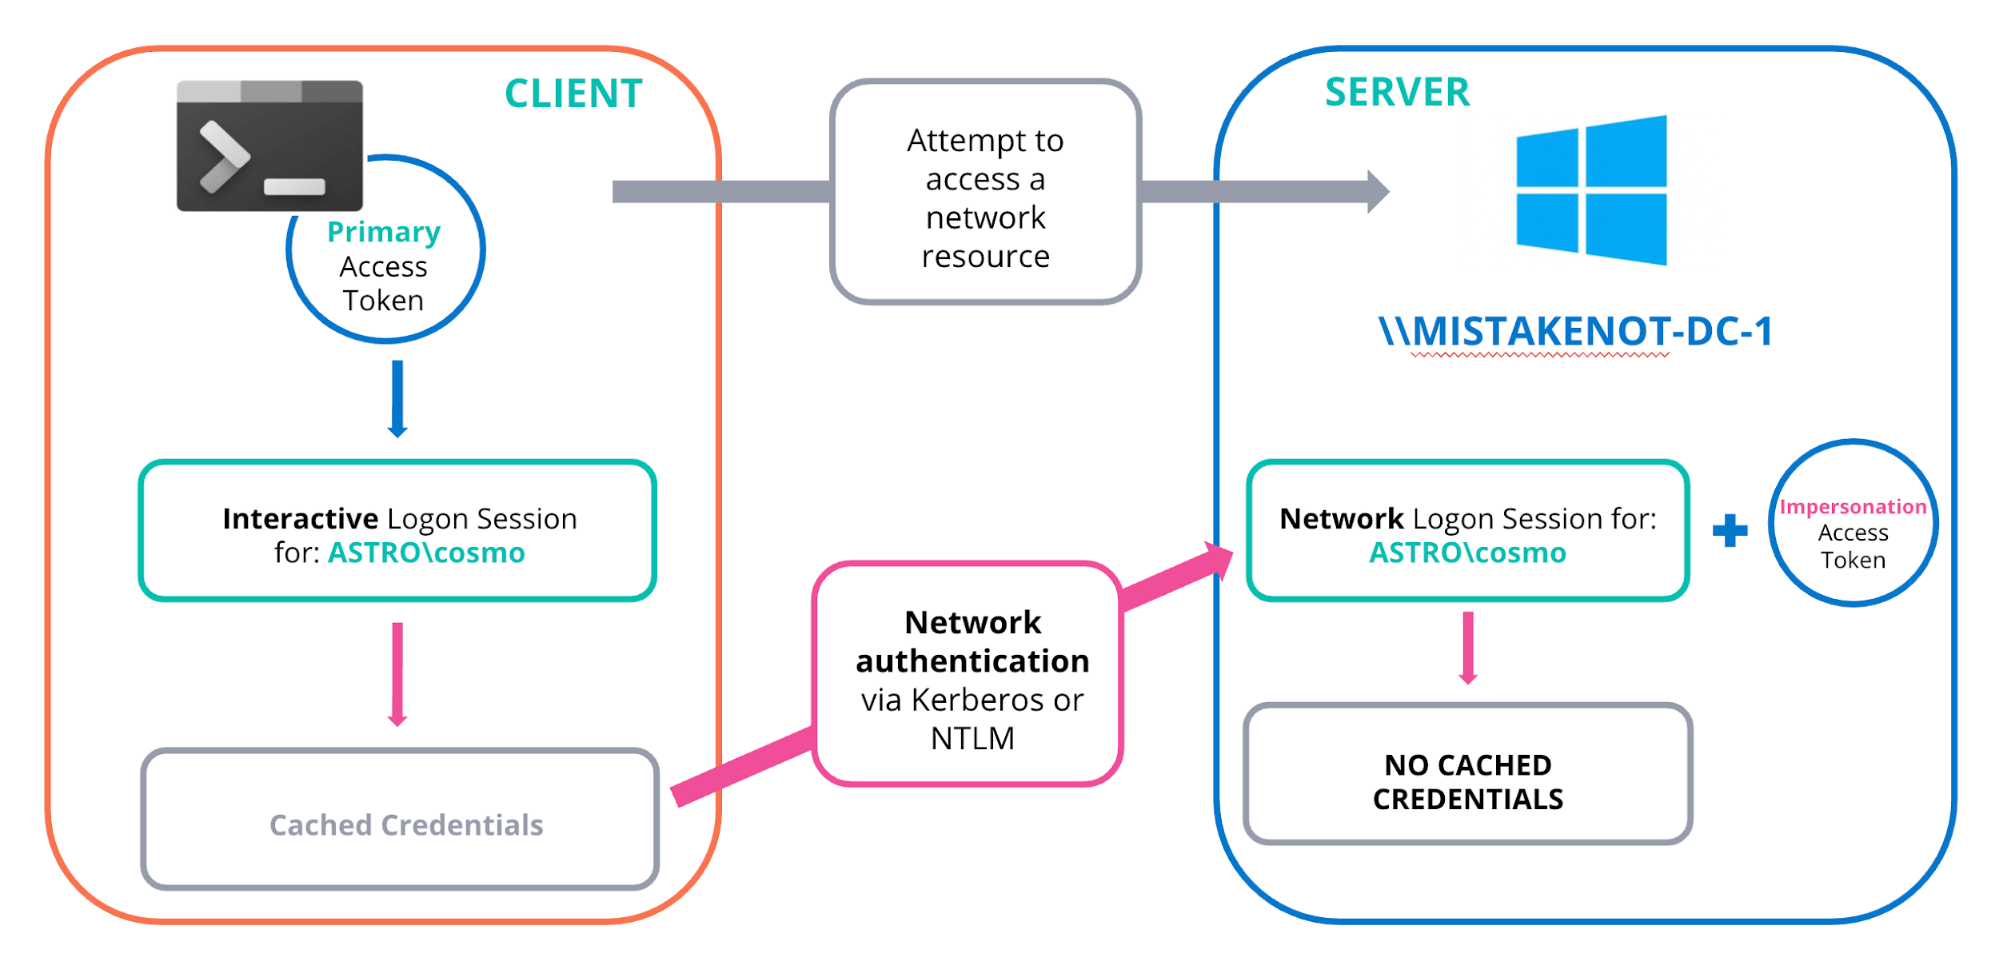
\includegraphics[width=\linewidth]{windows_knowledge/authorization/images/network-logon-tokens.png}
  \caption{Network Logon token}
    \label{fig:network-logon-token}
\end{figure}

In summary, from the perspective of a listening server process (say an SMB file server), the following steps must occur following a connection request from a remote client:
\begin{itemize}
    \item 
        The user is authenticated and a new logon session is created (\verb+NETWORK_ONLY+)
    \item 
        The server process is presented with a handle to an impersonation token which links back to the remote client’s new network logon session
    \item 
        The server can use this token to impersonate the client to perform work on their behalf
\end{itemize}

\subsection{Impresonation token}
An {\bf impersonation
token}\label{win:impresonation-token}\index{win!Impersonation Token} is an access token that is created to capture the security information of another agent. For example, if a server is doing a task on behalf of a client, the server is impersonating the client, and all operations will be performed under that client’s security context. Impersonation is simply the mechanism that allows a process to run by using the security credentials of another security object.

Keep in mind you may not add privileges to tokens after Windows generates them. Additionally, each sub-process generated by a thread inherited the parent process’s access token as-is. This is why there are times when a user may need to personate a token that belongs to them, but has a different set of privileges.

There are four impersonation levels:
\begin{itemize}
        \item \verb+SecurityAnonymous+ – The server cannot impersonate or identify the client.
        \item \verb+SecurityIdentification+ – With this, a server can get the identity and privileges of the client, but cannot impersonate the client.
        \item \verb+SecurityImpersonation+ – This impersonation level can impersonate the client’s security context on the local system.
        \item \verb+SecurityDelegation+ – The server can impersonate the client’s security context on remote systems.
\end{itemize}

Impersonation tokens can only be associated to threads, and they represent a client process's security subject. Impersonation tokens are usually created and associated to the current thread implicitly, by IPC mechanisms such as DCE RPC, DDE and named pipes.

\subsection{Restricted access token (filtered token)}
\label{win:filtered-token}

\href{https://docs.microsoft.com/en-us/windows/win32/secauthz/restricted-tokens}{Restricted
tokens} (also known as a filtered admin token) are a subset of primary or
impersonation tokens that have been modified to control privileges or
permissions. Restricted access tokens allow the system to remove privileges,
add deny-only access control entries, or perform other access rights changes.

Assuming User Account Control (UAC) is running during the initial token
creation process, LSA will attempt to identify if the user is a member of a
privileged group or has been granted a sensitive privilege using functionality
similar to the IsTokenRestricted function. Presence of a restricted SID will
result in a call to produce a new access token with reduced privileges.

\section{Security Reference Monitor}
The \emph{Security Reference Monitor
(SRM)}\label{win:SRM}\index{Windows!Security Reference Monitor (SRM)} is in charge to compare the security descriptors in the token with the security IDs for every file, folder, printer, or application that the user attempts to access. In this way, the access token provides a security context for the security principal’s actions on the computer.

For information about how access tokens are used in conjunction with logon and authentication in Windows, see the 
\url{https://docs.microsoft.com/en-us/previous-versions/windows/it-pro/windows-server-2003/cc758849(v=ws.10)?redirectedfrom=MSDN}{Access
Tokens Technical Reference}

\url{https://book.hacktricks.xyz/windows-hardening/windows-local-privilege-escalation/acls-dacls-sacls-aces}

\section{Integrity levels}
From Windows Vista, all protected objects are labeled with an integrity level. Most user and system files and registry keys on the system have a default label of “medium” integrity. The primary exception is a set of specific folders and files writeable by Internet Explorer 7 at Low integrity. Most processes run by standard users are labeled with medium integrity (even the ones started by a user inside the administrators group), and most services are labeled with System integrity. The root directory is protected by a high-integrity label.
Note that a process with a lower integrity level can’t write to an object with a higher integrity level.

There are several levels of integrity:
\begin{itemize}
    \item {\bf Untrusted}: processes that are logged on anonymously are automatically designated as Untrusted. Example: Chrome
    \item {\bf Low}: level used by default for interaction with the Internet. As long as Internet Explorer is run in its default state, Protected Mode, all files and processes associated with it are assigned the Low integrity level. Some folders, such as the Temporary Internet Folder, are also assigned the Low integrity level by default. However, note that a low integrity process is very restricted, it cannot write to the registry and it’s limited from writing to most locations in the current user’s profile. Example: Internet Explorer or Microsoft Edge
    \item {\bf Medium}: the context that most objects will run in. Standard users receive the Medium integrity level, and any object not explicitly designated with a lower or higher integrity level is Medium by default. Not that a user inside the Administrators group by default will use medium integrity levels.
    \item {\bf High}: Administrators are granted the High integrity level. This ensures that Administrators are capable of interacting with and modifying objects assigned Medium or Low integrity levels, but can also act on other objects with a High integrity level, which standard users can not do. Example: "Run as Administrator"
    \item {\bf System}: reserved for the system. The Windows kernel and core services are granted the System integrity level. Being even higher than the High integrity level of Administrators protects these core functions from being affected or compromised even by Administrators. Example: Services
    \item {\bf Installer}: special case and is the highest of all integrity levels. By virtue of being equal to or higher than all other WIC integrity levels, objects assigned the Installer integrity level are also able to uninstall all other objects.
\end{itemize}

You can get the integrity level of a process using \verb+Process Explorer+ from
Sysinternals, accessing the properties of the process and viewing the
"Security" tab.

You can also get your current integrity level using \verb+whoami /groups+

\subsection{Integrity Levels in File-system}
A object inside the file-system may need an minimum integrity level requirement and if a process doesn't have this integrity process it won't be able to interact with it.

\subsection{Integrity Levels in Binaries}

\begin{verbatim}
# show integrity level
icacls BINARY_PATH

# set integrity level
icacls BINARY_PATH /setintegritylevel LEVEL
\end{verbatim}

\subsection{Integrity Levels in Processes}

Not all files and folders have a minimum integrity level, but all processes are running under an integrity level. And similar to what happened with the file-system, if a process wants to write inside another process it must have at least the same integrity level. This means that a process with low integrity level can’t open a handle with full access to a process with medium integrity level.

Due to the restrictions commented in this and the previous section, from a security point of view, it's always recommended to run a process in the lower level of integrity possible.
